\documentclass[border=5pt]{standalone}
\usepackage{fontspec}
\usepackage{unicode-math}
\setmainfont{Noto Serif}
\setmathfont{STIXTwoMath-Regular.otf}
\usepackage{tikz}
\usetikzlibrary{arrows.meta,calc,decorations.pathmorphing,decorations.markings}
\tikzset{
 level/.style={draw=black,line width=.62pt,line cap=butt},
 axis/.style={draw=black,line width=.72pt,-{Latex[length=2.2mm,width=1.35mm]}},
 pump/.style={draw=black,line width=.8pt,-{Latex[length=2.4mm,width=1.5mm]}},
 curve/.style={draw=black,line width=1.35pt,line cap=round,line join=round},
 label/.style={font=\fontsize{14}{17}\selectfont,inner sep=2pt},
 link/.style={draw=black,line width=.8pt,line cap=round,line join=round},
 waveline/.style={link,decorate,decoration={snake,amplitude=.24mm,segment length=2.6mm,pre length=0mm,post length=0mm}}
}
\pagestyle{empty}
\begin{document}
% Figure 11.2. Source: author Fig.11.2, printed p.147.
% The smooth envelopes are schematic, not a measured Gaussian fit.
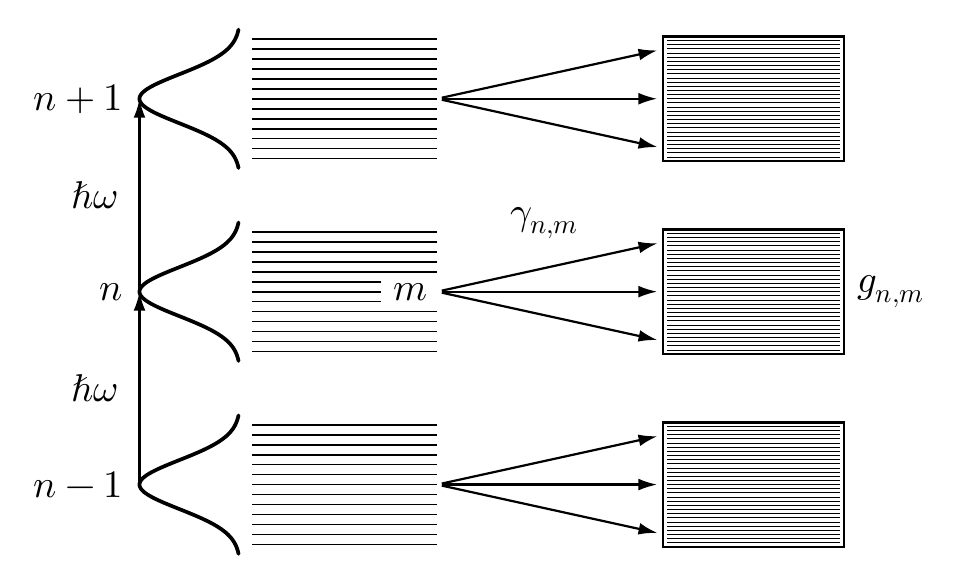
\begin{tikzpicture}[x=1cm,y=1cm]
\def\ZoneSpacing{2.45}
\def\ProfileSigma{.31}
\foreach \i/\nn in {0/{n-1},1/{n},2/{n+1}}{
 \pgfmathsetmacro{\cy}{1.02+\i*\ZoneSpacing}
 \coordinate (pump\i) at (0.10,\cy);
 \coordinate (out\i) at (3.88,\cy);
 \node[label,anchor=east] at (-.03,\cy) {$\nn$};
 \draw[curve,variable=\s,domain=-.88:.88,samples=180]
   plot ({1.38-1.28*exp(-.5*(\s/\ProfileSigma)^2)},{\cy+\s});
 \foreach \j in {0,...,12}{
  \pgfmathsetmacro{\yy}{\cy-.76+1.52*\j/12}
  \draw[level] (1.53,\yy) -- (3.88,\yy);
 }
 % The exit point lies exactly on the central zone level.
 \foreach \dy in {-.63,0,.63}{
  \draw[pump,shorten <=1.7pt,shorten >=2.1pt] (out\i) -- (6.75,{\cy+\dy});
 }
 % Continuum: the arrow tips stop at its left boundary, not inside the box.
 \draw[line width=.9pt] (6.75,{\cy-.79}) rectangle (9.05,{\cy+.79});
 \foreach \j in {0,...,28}{
  \pgfmathsetmacro{\yy}{\cy-.74+1.48*\j/28}
  \draw[line width=.30pt] (6.80,\yy) -- (9.00,\yy);
 }
}
\draw[pump] (pump0) -- (pump1);
\draw[pump] (pump1) -- (pump2);
\foreach \i in {0,1}{
 \node[label,anchor=east] at (-.10,{1.02+(\i+.5)*\ZoneSpacing}) {$\hbar\omega$};
}
% Opaque white backdrop masks level strokes without changing the physical state.
\node[label,fill=white,inner xsep=4.6pt,inner ysep=3pt] at (3.54,3.47) {$m$};
\node[label] at (5.25,4.34) {$\gamma_{n,m}$};
\node[label,anchor=west] at (9.14,3.47) {$g_{n,m}$};
\end{tikzpicture}
\end{document}
